\appendix
\chapter{Complete source-level typing rules}\label{app:source-rules}

This appendix lists the complete set of typing rules for the Veritas source language. Rules marked with $\star$ are also presented in Chapter~\ref{ch:impl}; they are repeated here for completeness.

\section*{Subsumption}

$$\frac{\phi; \Delta; \Gamma \vdash e \Rightarrow (\phi'; \Delta'; \tau_e) \quad \phi' \vdash \tau_e <: \tau}{\phi; \Delta; \Gamma \vdash e \Leftarrow \tau : (\phi'; \Delta')} \quad (\textsc{T-Sub})^\star$$

\section*{Subtyping}

$$\frac{}{\phi \vdash \tau <: \tau} \quad (\textsc{Sub-Refl})$$

$$\frac{}{\phi \vdash \textsf{int}(N) <: \textsf{int}} \quad (\textsc{Sub-Singleton-Int})$$

$$\frac{}{\phi \vdash \{x: \textsf{int} \mid P\} <: \textsf{int}} \quad (\textsc{Sub-Refine-Int})$$

$$\frac{\phi \vdash P[N/x]}{\phi \vdash \textsf{int}(N) <: \{x: \textsf{int} \mid P\}} \quad (\textsc{Sub-Singleton-Refine})^\star$$

$$\frac{\phi \wedge P_1 \vdash P_2}{\phi \vdash \{x: \textsf{int} \mid P_1\} <: \{x: \textsf{int} \mid P_2\}} \quad (\textsc{Sub-Refine-Refine})^\star$$

$$\frac{\phi \vdash \tau_1 <: \tau_2}{\phi \vdash [\tau_1; N] <: [\tau_2; N]} \quad (\textsc{Sub-Array})$$

$$\frac{\phi \vdash \tau <: \sigma}{\phi \vdash \textsf{master}(\tau) <: \sigma} \quad (\textsc{Sub-Master})$$

\section*{Literals and variables}

$$\frac{}{\phi; \Delta; \Gamma \vdash n \Rightarrow (\phi; \Delta; \textsf{int}(n))} \quad (\textsc{T-Int})$$

$$\frac{}{\phi; \Delta; \Gamma \vdash \textsf{true} \Rightarrow (\phi; \Delta; \textsf{bool})} \quad (\textsc{T-True})
  \qquad
  \frac{}{\phi; \Delta; \Gamma \vdash \textsf{false} \Rightarrow (\phi; \Delta; \textsf{bool})} \quad (\textsc{T-False})$$

$$\frac{(x: \tau) \in \Gamma}{\phi; \Delta; \Gamma \vdash x \Rightarrow (\phi; \Delta; \tau)} \quad (\textsc{T-Var-Imm})
  \qquad
  \frac{(x: \tau_c) \in \Delta}{\phi; \Delta; \Gamma \vdash x \Rightarrow (\phi; \Delta; \tau_c)} \quad (\textsc{T-Var-Mut})$$

\section*{Arithmetic}

$$
  \frac{
    \begin{array}{c}
      \phi_0; \Delta_0; \Gamma \vdash e_L \Rightarrow (\phi_1; \Delta_1; \tau_L) \quad \phi_1 \vdash \tau_L <: \textsf{int} \\
      \phi_1; \Delta_1; \Gamma \vdash e_R \Rightarrow (\phi_2; \Delta_2; \tau_R) \quad \phi_2 \vdash \tau_R <: \textsf{int} \\
      \tau_\textsf{res} = \textsf{join-op}(\textsf{aop}, \tau_L, \tau_R)
    \end{array}
  }{
    \phi_0; \Delta_0; \Gamma \vdash e_L \textsf{ aop } e_R \Rightarrow (\phi_2; \Delta_2; \tau_\textsf{res})
  } \quad (\textsc{T-Op})^\star
$$

\section*{Comparison and logical operators}

$$
  \frac{
    \begin{array}{c}
      \phi_0; \Delta_0; \Gamma \vdash e_L \Rightarrow (\phi_1; \Delta_1; \tau_L) \quad \phi_1 \vdash \tau_L <: \textsf{int} \\
      \phi_1; \Delta_1; \Gamma \vdash e_R \Rightarrow (\phi_2; \Delta_2; \tau_R) \quad \phi_2 \vdash \tau_R <: \textsf{int}
    \end{array}
  }{
    \phi_0; \Delta_0; \Gamma \vdash e_L \textsf{ cop } e_R \Rightarrow (\phi_2; \Delta_2; \textsf{bool})
  } \quad (\textsc{T-Cmp})
$$

$$
  \frac{
    \begin{array}{c}
      \phi_0; \Delta_0; \Gamma \vdash e_L \Rightarrow (\phi_1; \Delta_1; \tau_L) \quad \phi_1 \vdash \tau_L <: \textsf{bool} \\
      \phi_1; \Delta_1; \Gamma \vdash e_R \Rightarrow (\phi_2; \Delta_2; \tau_R) \quad \phi_2 \vdash \tau_R <: \textsf{bool}
    \end{array}
  }{
    \phi_0; \Delta_0; \Gamma \vdash e_L \textsf{ lop } e_R \Rightarrow (\phi_2; \Delta_2; \textsf{bool})
  } \quad (\textsc{T-Lop})
$$

\section*{Array creation}

$$
  \frac{
    \begin{array}{c}
      \phi_0; \Delta_0; \Gamma \vdash e_\textsf{val} \Rightarrow (\phi_1; \Delta_1; \tau_\textsf{val})   \\
      \phi_1; \Delta_1; \Gamma \vdash e_\textsf{size} \Rightarrow (\phi_2; \Delta_2; \tau_\textsf{size}) \\
      \phi_2 \vdash \tau_\textsf{size} <: \textsf{int} \quad N = \textsf{val}(\tau_\textsf{size})
    \end{array}
  }{
    \phi_0; \Delta_0; \Gamma \vdash [e_\textsf{val}; e_\textsf{size}] \Rightarrow (\phi_2; \Delta_2; [\tau_\textsf{val}; N])
  } \quad (\textsc{T-Array-Create})
$$

\section*{Array indexing}

$$
  \frac{
    \begin{array}{c}
      (x: [\tau_\textsf{elem}; N]) \in (\Gamma \cup \Delta_0)                                                               \\
      \phi_0; \Delta_0; \Gamma \vdash e_i \Rightarrow (\phi_1; \Delta_1; \tau_i) \quad \phi_1 \vdash \tau_i <: \textsf{int} \\
      \phi_1 \wedge \textsf{prop}(\tau_i) \vdash 0 \le \textsf{val}(\tau_i) < N \quad \text{(Bounds proof)}
    \end{array}
  }{
    \phi_0; \Delta_0; \Gamma \vdash x[e_i] \Rightarrow (\phi_1; \Delta_1; \tau_\textsf{elem})
  } \quad (\textsc{T-Array-Idx})^\star
$$

\section*{Conditional expressions}

$$
  \frac{
    \begin{array}{c}
      \phi_0; \Delta_0; \Gamma \vdash e_\textsf{cond} \Rightarrow (\phi_1; \Delta_1; \tau_c) \quad \phi_1 \vdash \tau_c <: \textsf{bool} \\
      \phi_1 \wedge \textsf{prop}(\tau_c); \Delta_1; \Gamma \vdash B \Rightarrow (\phi_2; \Delta_2; \tau_2)                              \\
      \phi_1 \wedge \neg \textsf{prop}(\tau_c); \Delta_1; \Gamma \vdash B' \Rightarrow (\phi_3; \Delta_3; \tau_3)                        \\
      (\phi_\textsf{join}, \Delta_\textsf{join}, \tau_\textsf{join}) = \textsf{join}(\phi_2, \Delta_2, \tau_2, \phi_3, \Delta_3, \tau_3)
    \end{array}
  }{
    \phi_0; \Delta_0; \Gamma \vdash (\textsf{if } e_\textsf{cond}\; B \textsf{ else } B') \Rightarrow (\phi_\textsf{join}; \Delta_\textsf{join}; \tau_\textsf{join})
  } \quad (\textsc{T-If-Expr})^\star
$$

\section*{Function calls}

$$
  \frac{
    \begin{array}{c}
      \Sigma_F(f) = ( (x_i:\tau_i)_{i=1}^k \rightarrow \tau_\textsf{ret}\; \textsf{requires } P_\textsf{req} ) \\
      \phi_0; \Delta_0; \Gamma \vdash \vec{e} \Rightarrow (\phi_k; \Delta_k; \vec{\sigma})                     \\
      \forall i \in 1..k,\; \phi_k \vdash \sigma_i <: \tau_i                                                   \\
      \phi_k \wedge \textsf{prop}(\vec{\sigma}) \vdash P_\textsf{req}[\textsf{val}(\vec{\sigma}) / \vec{x}] \quad \text{(Precondition proof)}
    \end{array}
  }{
    \phi_0; \Delta_0; \Gamma \vdash f(\vec{e}) \Rightarrow (\phi_k; \Delta_k; \tau_\textsf{ret})
  } \quad (\textsc{T-Call})^\star
$$

\section*{Blocks and bindings}

$$
  \frac{}{\phi; \Delta; \Gamma \vdash \cdot : (\phi; \Delta; \Gamma)} \quad (\textsc{T-Block-Empty})
$$

$$
  \frac{
    \phi_0; \Delta_0; \Gamma_0 \vdash S : (\phi_1; \Delta_1; \Gamma_1) \quad \phi_1; \Delta_1; \Gamma_1 \vdash B : (\phi_2; \Delta_2; \Gamma_2)
  }{
    \phi_0; \Delta_0; \Gamma_0 \vdash (S\; B) : (\phi_2; \Delta_2; \Gamma_2)
  } \quad (\textsc{T-Block-Seq})
$$

$$\frac{\phi_0; \Delta_0; \Gamma \vdash e \Leftarrow \tau : (\phi_1; \Delta_1)}{\phi_0; \Delta_0; \Gamma \vdash (\textsf{let } x:\tau = e;) : (\phi_1; \Delta_1; \Gamma, x:\tau)} \quad (\textsc{T-Let})$$

$$\frac{\phi_0; \Delta_0; \Gamma \vdash e \Leftarrow \tau : (\phi_1; \Delta_1)}{\phi_0; \Delta_0; \Gamma \vdash (\textsf{let mut } x:\tau = e;) : (\phi_1; (\Delta_1, x:\tau); \Gamma)} \quad (\textsc{T-Let-Mut})$$

\section*{Array assignment}

$$
  \frac{
    \begin{array}{c}
      (x: [\tau_\textsf{elem}; N]) \in \Delta_0                                                                                 \\
      \phi_0; \Delta_0; \Gamma \vdash e_i \Rightarrow (\phi_1; \Delta_1; \tau_i) \quad \phi_1 \vdash \tau_i <: \textsf{int}     \\
      \phi_1; \Delta_1; \Gamma \vdash e \Rightarrow (\phi_2; \Delta_2; \tau_v) \quad \phi_2 \vdash \tau_v <: \tau_\textsf{elem} \\
      \phi_2 \wedge \textsf{prop}(\tau_i) \vdash 0 \le \textsf{val}(\tau_i) < N \quad \text{(Bounds proof)}
    \end{array}
  }{
    \phi_0; \Delta_0; \Gamma \vdash (x[e_i] = e;) : (\phi_2; \Delta_2; \Gamma)
  } \quad (\textsc{T-Array-Assign})
$$

\section*{Assignment}

$$
  \frac{
    \begin{array}{c}
      (x: \tau_m) \in \Delta_0                                                 \\
      \phi_0; \Delta_0; \Gamma \vdash e \Rightarrow (\phi_1; \Delta_1; \tau_e) \\
      \phi_1 \vdash \tau_e <: \tau_m
    \end{array}
  }{
    \phi_0; \Delta_0; \Gamma \vdash (x = e;) : (\phi_1; \Delta_1[x \mapsto (\tau_e, \tau_m)]; \Gamma)
  } \quad (\textsc{T-Assign})^\star
$$

\section*{For loop}

$$
  \frac{
    \begin{array}{c}
      \phi_0 \wedge P_I[e_\textsf{start}/i] \quad \text{(Invariant holds on entry)}                                                                   \\
      \phi_0 \wedge P_I \wedge e_\textsf{start} \le i < e_\textsf{end};\; \Delta_0;\; (\Gamma, i: \textsf{int}) \vdash B : (\phi_1; \Delta_1; \Gamma) \\
      \phi_1 \vdash P_I[(i+1)/i] \quad \text{(Invariant preserved by body)}
    \end{array}
  }{
    \phi_0; \Delta_0; \Gamma \vdash (\textsf{for } i \textsf{ in } e_\textsf{start}..e_\textsf{end}\;\{B\}) : (\phi_0 \wedge P_I; \Delta_0; \Gamma)
  } \quad (\textsc{T-For})^\star
$$

\noindent where $P_I$ is the invariant proposition (or $\top$ if no invariant is specified).

\section*{Return}

$$
  \frac{
    \begin{array}{c}
      \phi_0; \Delta_0; \Gamma \vdash e \Rightarrow (\phi_1; \Delta_1; \tau_e) \quad \phi_1 \vdash \tau_e <: \tau_\textsf{ret} \\
      \phi_1 \vdash P_\textsf{ens}[e/\mathtt{result}] \quad \text{(Postcondition proof)}
    \end{array}
  }{
    \phi_0; \Delta_0; \Gamma \vdash (\textsf{return } e;) : (\phi_1; \Delta_1; \Gamma)
  } \quad (\textsc{T-Return})^\star
$$

\section*{If-statement and while loop}

$$
  \frac{
    \begin{array}{c}
      \phi_0; \Delta_0; \Gamma \vdash e_\textsf{cond} \Rightarrow (\phi_1; \Delta_1; \tau_c) \quad \phi_1 \vdash \tau_c <: \textsf{bool} \\
      \phi_1 \wedge \textsf{prop}(\tau_c); \Delta_1; \Gamma \vdash B : (\phi_2; \Delta_2; \Gamma)                                        \\
      \phi_1 \wedge \neg \textsf{prop}(\tau_c); \Delta_1; \Gamma \vdash B' : (\phi_3; \Delta_3; \Gamma)                                  \\
      (\phi_\textsf{join}, \Delta_\textsf{join}) = \textsf{join}(\phi_2, \Delta_2, \phi_3, \Delta_3)
    \end{array}
  }{
    \phi_0; \Delta_0; \Gamma \vdash (\textsf{if } e_\textsf{cond}\; B \textsf{ else } B') : (\phi_\textsf{join}; \Delta_\textsf{join}; \Gamma)
  } \quad (\textsc{T-If-Stmt})
$$

$$
  \frac{
    \begin{array}{c}
      \phi_0; \Delta_0; \Gamma \vdash e_\textsf{cond} \Rightarrow (\phi_1; \Delta_1; \tau_c) \quad \phi_1 \vdash \tau_c <: \textsf{bool} \\
      \phi_0 \vdash \phi_I \quad \text{(Invariant holds on entry)}                                                                       \\
      \phi_I \wedge \textsf{prop}(\tau_c);\; \Delta_0;\; \Gamma \vdash B : (\phi_2; \Delta_2; \Gamma)                                    \\
      \phi_2; \Delta_2 \vdash \phi_I \quad \text{(Invariant preserved by body)}
    \end{array}
  }{
    \phi_0; \Delta_0; \Gamma \vdash (\textsf{while } e_\textsf{cond}\;\{B\}) : (\phi_I \wedge \neg\textsf{prop}(\tau_c); \Delta_0; \Gamma)
  } \quad (\textsc{T-While})
$$

\chapter{Complete DTAL typing rules}\label{app:dtal-rules}

This appendix lists the complete set of typing rules implemented by the DTAL verifier. Each rule has the form $\Phi; \Gamma \vdash \textsf{instr} \Rightarrow \Gamma'$, where $\Phi$ is the constraint context, $\Gamma$ maps registers to types, and $\Gamma'$ is the updated register map. We write $\textsf{idx}(\tau)$ for the index expression extracted from a type (e.g., $\textsf{idx}(\textsf{int}(e)) = e$). Rules marked with $\star$ are also presented in Chapter~\ref{ch:impl}.

\section*{Data movement}

$$
  \frac{}{\Phi; \Gamma \vdash \textsf{mov } r_d, n \Rightarrow \Gamma[r_d \mapsto \textsf{int}(n)]} \quad (\textsc{D-MovImm})^\star
$$

$$
  \frac{\Gamma(r_s) = \tau}{\Phi; \Gamma \vdash \textsf{mov } r_d, r_s \Rightarrow \Gamma[r_d \mapsto \tau]} \quad (\textsc{D-MovReg})
$$

$$
  \frac{
    \begin{array}{c}
      \Gamma(r_b) = [\tau; N] \quad \Phi \vdash 0 \le \textsf{idx}(\Gamma(r_i)) < N
    \end{array}
  }{\Phi; \Gamma \vdash \textsf{load } r_d, [r_b, r_i] \Rightarrow \Gamma[r_d \mapsto \tau]} \quad (\textsc{D-Load})^\star
$$

$$
  \frac{
    \begin{array}{c}
      \Gamma(r_b) = [\tau; N] \quad \Phi \vdash 0 \le \textsf{idx}(\Gamma(r_i)) < N \\
      v' = v + 1 \quad \text{(fresh array version)}
    \end{array}
  }{\Phi; \Gamma \vdash \textsf{store } [r_b, r_i], r_s \Rightarrow \Gamma} \quad (\textsc{D-Store})
$$

\noindent After a store, the verifier emits two axioms into $\Phi$: a \textit{write axiom} ($\textsf{select}(\mathit{arr}_{v'}, e_i) = e_s$) and a \textit{frame axiom} ($\forall k.\; k \ne e_i \Rightarrow \textsf{select}(\mathit{arr}_{v'}, k) = \textsf{select}(\mathit{arr}_v, k)$), where $v$ and $v'$ are the old and new array versions.

\section*{Arithmetic}

$$
  \frac{
    \Gamma(r_1) = \textsf{int}(e_1) \quad \Gamma(r_2) = \textsf{int}(e_2)
  }{\Phi; \Gamma \vdash \textsf{binop}_\oplus\; r_d, r_1, r_2 \Rightarrow \Gamma[r_d \mapsto \textsf{int}(e_1 \oplus e_2)]} \quad (\textsc{D-BinOp-Singleton})^\star
$$

$$
  \frac{
    \Gamma(r_1) = \{a\!:\!\textsf{int} \mid \varphi_1\} \quad \Gamma(r_2) = \{b\!:\!\textsf{int} \mid \varphi_2\}
  }{\Phi; \Gamma \vdash \textsf{binop}_\oplus\; r_d, r_1, r_2 \Rightarrow \Gamma[r_d \mapsto \exists c.\; \textsf{int}(c) \;\mathbf{where}\; \exists a,b.\; \varphi_1 \wedge \varphi_2 \wedge c = a \oplus b]} \quad (\textsc{D-BinOp-Refined})^\star
$$

$$
  \frac{
    \Gamma(r_s) = \textsf{int}(e)
  }{\Phi; \Gamma \vdash \textsf{addimm } r_d, r_s, n \Rightarrow \Gamma[r_d \mapsto \textsf{int}(e + n)]} \quad (\textsc{D-AddImm})
$$

$$
  \frac{
    \Gamma(r_s) = \tau \quad \tau <: \textsf{bool}
  }{\Phi; \Gamma \vdash \textsf{not } r_d, r_s \Rightarrow \Gamma[r_d \mapsto \textsf{bool}]} \quad (\textsc{D-Not})
$$

\section*{Comparison and branching}

$$
  \frac{
    \Gamma(r_1) = \tau_1 \quad \Gamma(r_2) = \tau_2
  }{\Phi; \Gamma \vdash \textsf{cmp } r_1, r_2 \Rightarrow \Gamma \quad \text{(records operands } \textsf{idx}(\tau_1), \textsf{idx}(\tau_2)\text{)}} \quad (\textsc{D-Cmp})
$$

$$
  \frac{
    \Gamma(r_1) = \tau_1
  }{\Phi; \Gamma \vdash \textsf{cmp } r_1, n \Rightarrow \Gamma \quad \text{(records operands } \textsf{idx}(\tau_1), n\text{)}} \quad (\textsc{D-CmpImm})
$$

$$
  \frac{}{\Phi; \Gamma \vdash \textsf{setcc } r_d, \textit{cond} \Rightarrow \Gamma[r_d \mapsto \textsf{bool}]} \quad (\textsc{D-SetCC})
$$

$$
  \frac{
    \text{last cmp operands: } e_1, e_2
  }{\Phi; \Gamma \vdash \textsf{branch } \textit{cond}\; L \Rightarrow \Gamma \quad \text{with } \Phi' = \Phi \wedge \neg(e_1 \textit{ cond } e_2) \text{ (fall-through)}} \quad (\textsc{D-Branch})^\star
$$

\noindent The taken edge to $L$ carries $\Phi \wedge (e_1 \textit{ cond } e_2)$.

\section*{Stack and allocation}

$$
  \frac{\Gamma(r_s) = \tau}{\Phi; \Gamma \vdash \textsf{push } r_s \Rightarrow \Gamma \quad \text{(push } \tau \text{ onto typed stack)}} \quad (\textsc{D-Push})
$$

$$
  \frac{S = \tau :: S'}{\Phi; \Gamma \vdash \textsf{pop } r_d \Rightarrow \Gamma[r_d \mapsto \tau] \quad \text{(pop from typed stack)}} \quad (\textsc{D-Pop})
$$

$$
  \frac{}{\Phi; \Gamma \vdash \textsf{alloca } r_d, n \Rightarrow \Gamma[r_d \mapsto [\textsf{int}; n]]} \quad (\textsc{D-Alloca})
$$

\noindent After allocation, the verifier adds a zero-initialisation axiom: $\forall k \in [0, n).\; \textsf{select}(\mathit{arr}_0, k) = 0$.

\section*{Annotations}

$$
  \frac{
    \Gamma(r) = \tau_\textsf{derived} \quad \Phi \vdash \tau_\textsf{derived} <: \tau_\textsf{ann}
  }{\Phi; \Gamma \vdash \textsf{type } r: \tau_\textsf{ann}} \quad (\textsc{D-TypeAnn})
$$

\noindent The verifier derives the register's type independently and checks it is compatible with the compiler's annotation. If the annotation is more precise (e.g., a singleton vs.\ the derived existential), the verifier checks that the derived type implies the annotation under $\Phi$.

$$
  \frac{
    \Phi \vdash C
  }{\Phi; \Gamma \vdash \textsf{assert } C \Rightarrow \Gamma \quad \text{(add } C \text{ to } \Phi\text{)}} \quad (\textsc{D-Assert})
$$

\noindent The verifier checks that the constraint $C$ is provable from the current $\Phi$ before adding it.

\section*{Function calls}

$$
  \frac{
    \begin{array}{c}
      \Sigma(f) = (\vec{x}:\vec{\tau}) \rightarrow \tau_\textsf{ret} \;\textsf{requires } P_\textsf{req} \;\textsf{ensures } P_\textsf{ens} \\
      \Phi \vdash P_\textsf{req}[\overline{r_i / x_i}]
    \end{array}
  }{\Phi; \Gamma \vdash \textsf{call } f \Rightarrow \Gamma[r_0 \mapsto \tau_\textsf{ret}] \quad \text{(add } P_\textsf{ens}[\overline{r_i / x_i}] \text{ to } \Phi\text{)}} \quad (\textsc{D-Call})
$$

\noindent The precondition is checked against $\Phi$ after substituting physical parameter registers for formal parameters. The postcondition (with \texttt{result} replaced by $r_0$) is assumed in $\Phi$ after the call.

\section*{Physical instructions (post-regalloc)}

The following instructions appear only after register allocation and are verified for basic consistency:

\begin{itemize}
  \item \textbf{D-Cqo}: Sign-extends \texttt{rax} into \texttt{rdx:rax}. The type of \texttt{rdx} is set to the type of \texttt{rax}.
  \item \textbf{D-Idiv}: Divides \texttt{rdx:rax} by the source register. Both \texttt{rax} (quotient) and \texttt{rdx} (remainder) receive type $\textsf{int}$.
  \item \textbf{D-SpillStore}: Records the type stored at a stack offset.
  \item \textbf{D-SpillLoad}: Checks that the loaded type matches what was previously stored at that offset.
  \item \textbf{D-Prologue / D-Epilogue}: Structural markers verified at the function level.
\end{itemize}

% \chapter{Pipeline correspondence tables}\label{app:pipeline-correspondence}
%
% \begin{table}[h]
%   \centering
%   \scriptsize
%   \begin{tabular}{p{0.27\textwidth} p{0.32\textwidth} p{0.32\textwidth}}
%     \hline
%     \textbf{Source construct} & \textbf{TIR representation} & \textbf{DTAL representation} \\
%     \hline
%     Integer / boolean literal
%     & $\rho := n : \tau$
%     & \texttt{mov} into a register with a singleton or base type annotation \\
%     Variable use
%     & Read the virtual register currently bound to the source variable
%     & Use the corresponding virtual or physical register in later instructions \\
%     Immutable binding \texttt{let x:T = e}
%     & Lower $e$ to a fresh virtual register and bind $x$ to that register
%     & Instructions computing $e$, with the result type carried on the destination register \\
%     Mutable assignment \texttt{x = e}
%     & Lower $e$ to a fresh virtual register and update the variable-to-register map
%     & Ordinary computation instructions; SSA reassignment has already been made explicit in TIR \\
%     Arithmetic expression \texttt{e1 op e2}
%     & \texttt{BinOp \{ dst, op, lhs, rhs, ty \}}
%     & Arithmetic instruction such as \texttt{add}, \texttt{sub}, or \texttt{mul}, carrying the derived result type \\
%     Comparison expression
%     & \texttt{BinOp} or branch condition register with true/false constraints
%     & \texttt{cmp} followed by \texttt{setcc} or conditional branch; branch facts refine the verifier context \\
%     Conditional expression / statement
%     & \texttt{Branch \{ cond, true\_target, false\_target, true\_constraint, false\_constraint \}} plus merge phi nodes
%     & \texttt{cmp}/branch instructions and labelled blocks with checked entry states \\
%     Loop
%     & Header/body/exit blocks, loop-carried phi nodes, and translated invariant assertions
%     & Labelled blocks with \texttt{.entry}, \texttt{.assume}, branches, and \texttt{.assert} constraints \\
%     Function call
%     & \texttt{Call \{ dst?, func, args, arg\_types, result\_ty \}}
%     & Argument registers following the calling convention, \texttt{call}, precondition check, and postcondition context update \\
%     Return
%     & \texttt{Return \{ value? \}}
%     & Move result to the return register where needed, then \texttt{ret} \\
%     Array creation
%     & Allocation or initialisation instructions, depending on the source form
%     & Stack/runtime allocation support plus array type information and initialisation facts \\
%     Array read \texttt{a[i]}
%     & \texttt{ArrayLoad \{ dst, base, index, element\_ty, bounds\_constraint \}}
%     & Address computation plus typed \texttt{load}; verifier proves the bounds constraint \\
%     Array write \texttt{a[i] = e}
%     & \texttt{ArrayStore \{ base, index, value, bounds\_constraint \}}
%     & Address computation plus typed \texttt{store}; verifier proves the bounds constraint \\
%     Function precondition
%     & Function-level constraint and call-site proof obligation
%     & \texttt{.precondition}; verifier checks callers establish the required constraint \\
%     Function postcondition
%     & Function-level result constraint
%     & \texttt{.postcondition}; verifier adds the instantiated fact after a verified call \\
%     Loop invariant / assertion
%     & \texttt{AssertConstraint \{ constraint \}}
%     & \texttt{.assert}; checked before being added to the DTAL constraint context \\
%     Path assumption
%     & \texttt{AssumeConstraint \{ constraint \}}
%     & \texttt{.assume}; contributes to the declared block-entry context \\
%     SSA join
%     & \texttt{PhiNode \{ dst, ty, incoming, existential\_constraint \}}
%     & Edge copies plus block-entry type state; existential facts preserve joined refinement information \\
%     \hline
%   \end{tabular}
%   \caption{Correspondence between representative source constructs, TIR forms, and verifier-facing DTAL forms.}
%   \label{tab:source-tir-dtal-correspondence}
% \end{table}

\chapter{Evaluation tables}\label{app:evaluation-supplementary}

\begin{figure}[h]
  \centering
  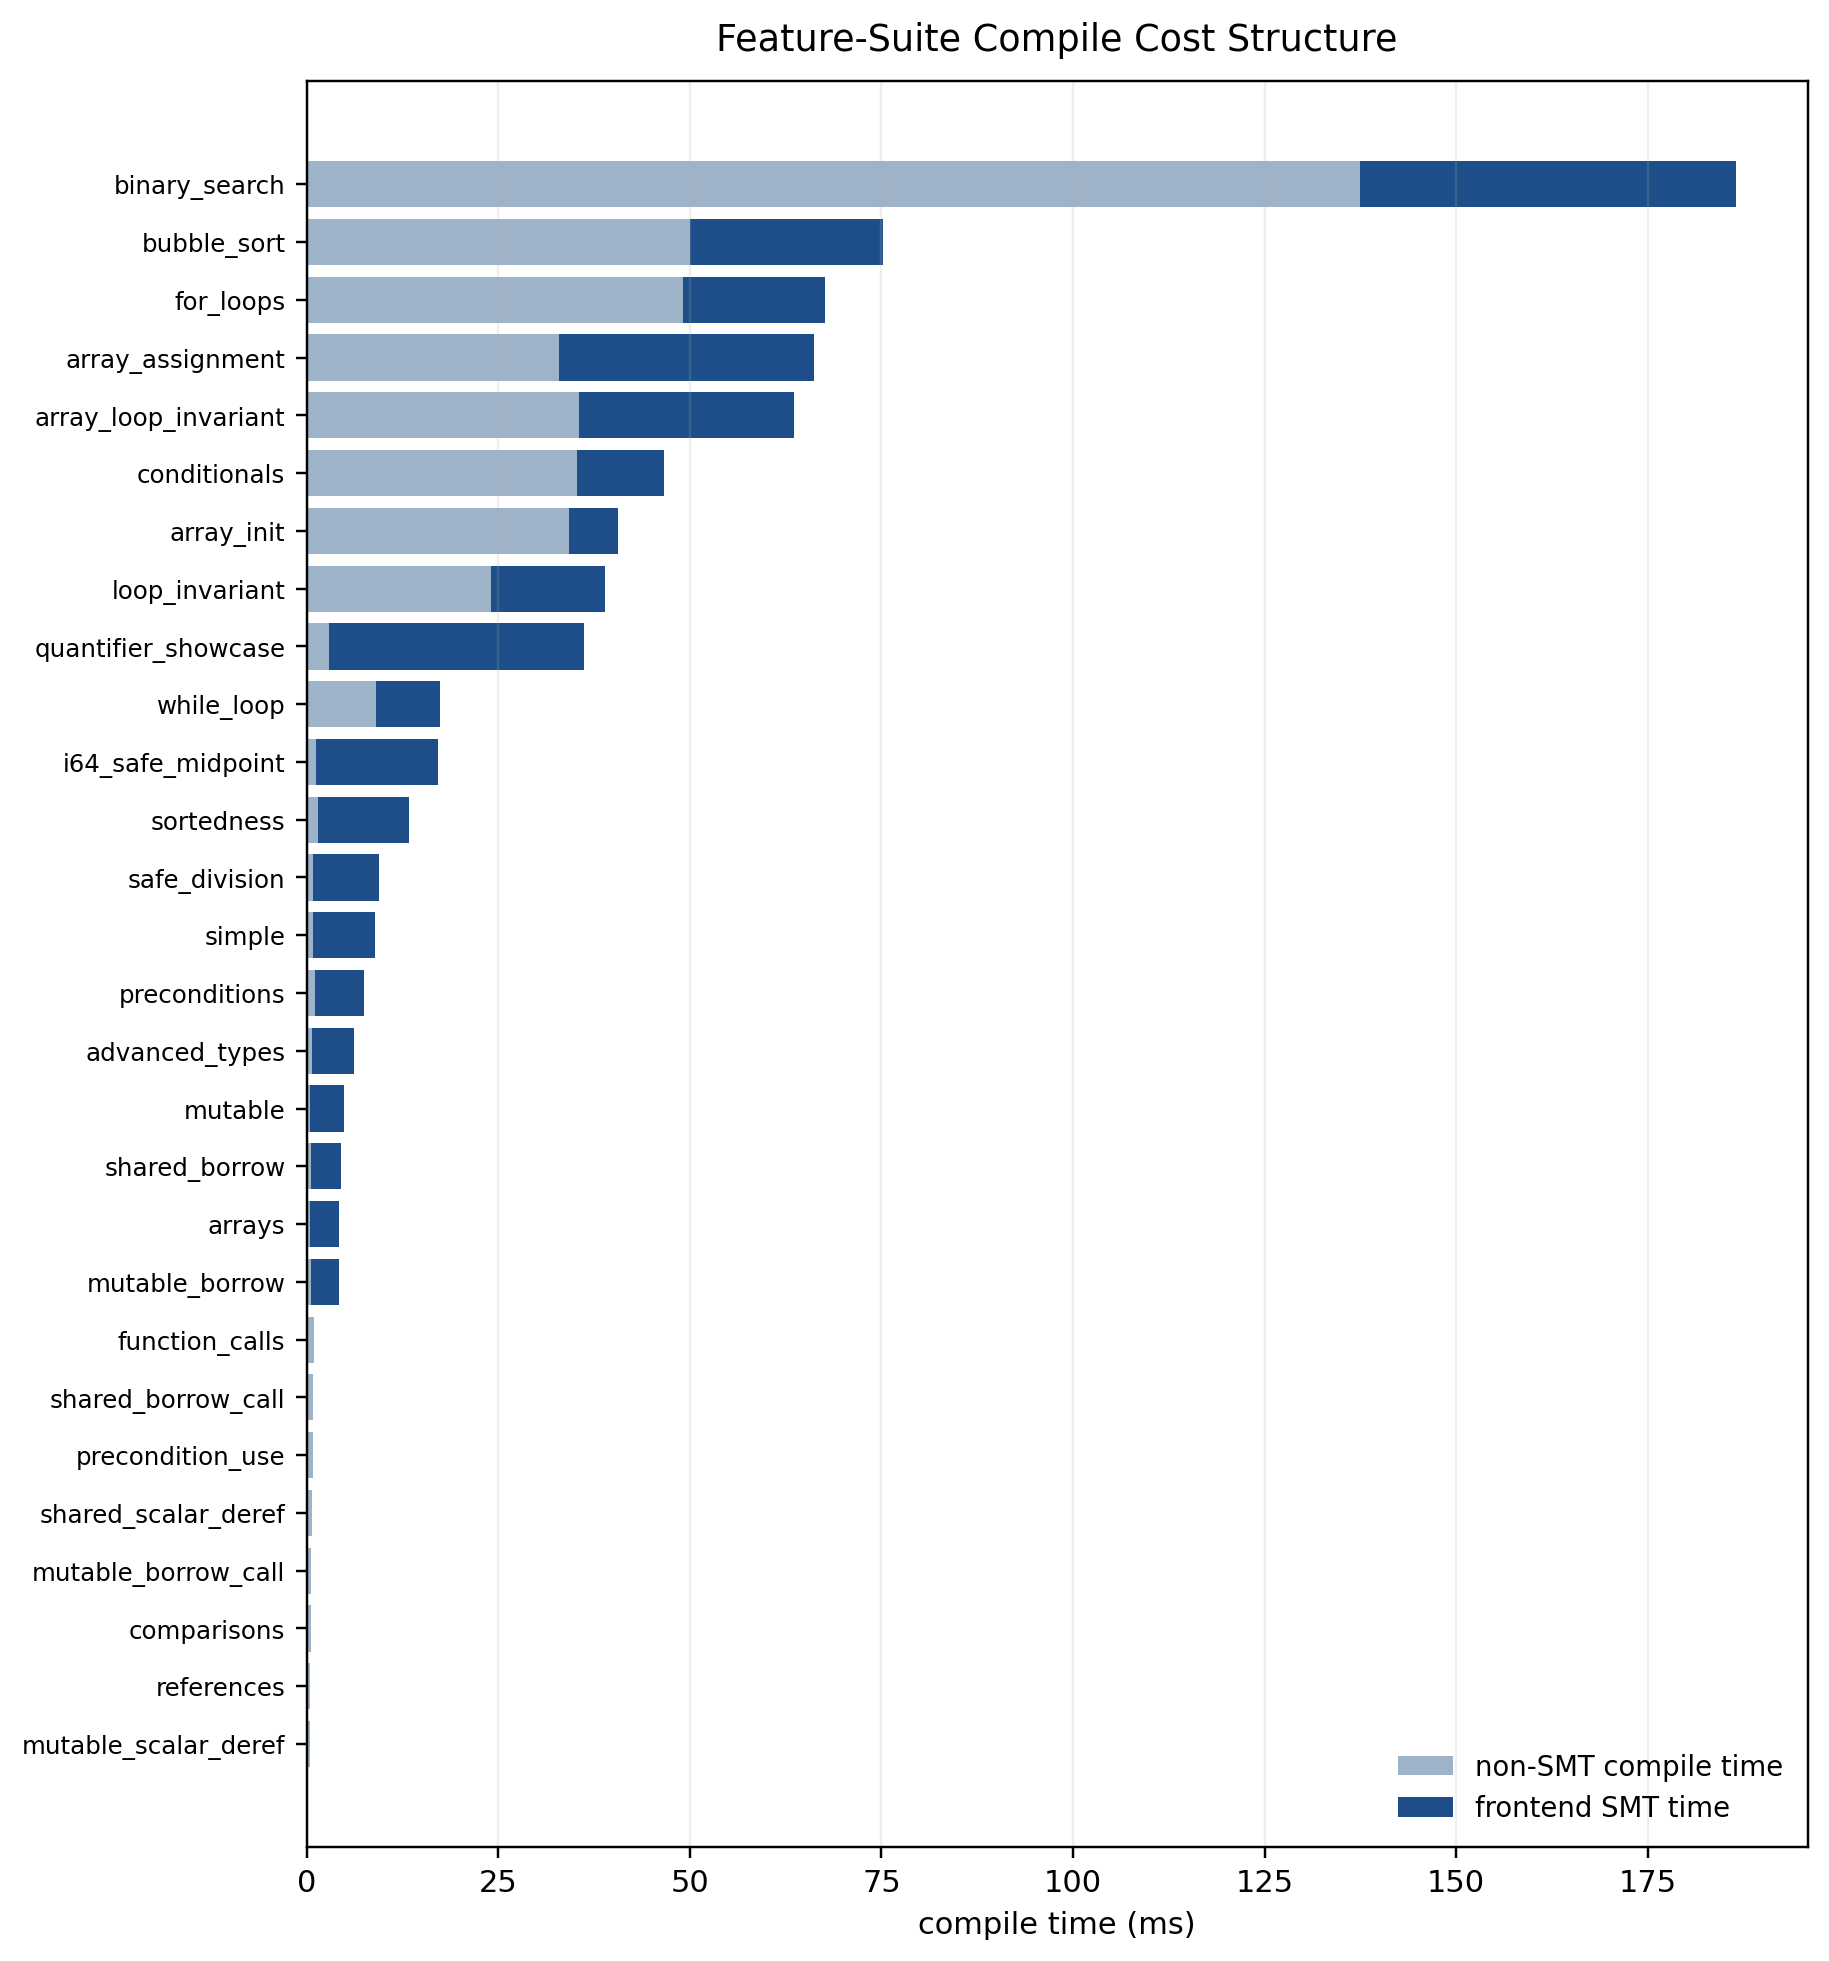
\includegraphics[width=0.82\textwidth]{figures/chapter4_feature_suite_compile_cost.png}
  \caption{Compile-cost structure across the complete curated feature suite.}
  \label{fig:feature-suite-compile-cost-full}
\end{figure}

\begin{table}[h]
  \centering
  \scriptsize
  \begin{tabular}{p{0.17\textwidth} p{0.17\textwidth} p{0.31\textwidth} p{0.25\textwidth}}
    \hline
    \textbf{Kernel} & \textbf{Fixed \texttt{MEDIUM} params} & \textbf{Program / algorithm}                                                       & \textbf{Main features exercised}                                                                     \\
    \hline
    Floyd--Warshall & \texttt{N=500}                        & All-pairs shortest paths via dynamic programming over a weighted graph matrix.     & Nested loops, fixed-size 2D arrays, arithmetic updates, regular indexed mutation                     \\
    Jacobi-1D       & \texttt{N=400}, \texttt{T=100}        & One-dimensional iterative stencil update over an array across repeated time steps. & Structured loop nests, fixed-size arrays, repeated affine indexing, arithmetic recurrence            \\
    Jacobi-2D       & \texttt{N=250}, \texttt{T=100}        & Two-dimensional iterative stencil computation over a grid.                         & Nested loops, fixed-size 2D arrays, neighbourhood indexing, arithmetic recurrence                    \\
    Seidel-2D       & \texttt{N=400}, \texttt{T=100}        & In-place two-dimensional smoothing stencil over a grid.                            & Nested loops, in-place array mutation, affine neighbour access, arithmetic accumulation              \\
    MVT             & \texttt{N=400}                        & Matrix-vector and transposed-matrix-vector multiplication kernel.                  & Fixed-size arrays, matrix/vector indexing, arithmetic accumulation, sequential imperative loops      \\
    ATAX            & \texttt{M=390}, \texttt{N=410}        & Matrix-transpose-times-vector style kernel with intermediate accumulation.         & Matrix/vector array reasoning, multiple loop phases, arithmetic accumulation, indexed mutation       \\
    GESUMMV         & \texttt{N=250}                        & Scalar-weighted sum of two matrix-vector products.                                 & Fixed-size arrays, linear-algebra style arithmetic, nested loops, deterministic numeric accumulation \\
    \hline
  \end{tabular}
  \caption{PolyBench-style kernels used in the Veritas evaluation, with their
    fixed \texttt{MEDIUM}-class parameters, algorithmic role, and the main
    language/compiler features they exercise.}
  \label{tab:polybench-kernels}
\end{table}

\begin{table}[h]
  \centering
  \small
  \begin{tabular}{p{0.33\textwidth} c c p{0.4\textwidth}}
    \hline
    \textbf{Feature}                           & \textbf{Xi--Harper} & \textbf{Veritas} & \textbf{Notes}                                                                                                               \\
    \hline
    Independent low-level verification         & Yes                 & Yes              & Core architectural idea shared by both systems.                                                                              \\
    Dependent block / label state types        & Yes                 & Yes              & Xi--Harper uses typed labels; Veritas uses \texttt{.entry} plus \texttt{.assume}.                                            \\
    Singleton integer types \texttt{int(x)}    & Yes                 & Yes              & Present in both; Veritas derives symbolic index expressions similarly.                                                       \\
    Size-indexed array types                   & Yes                 & Yes              & Xi--Harper uses \texttt{int array(m)}; Veritas uses array types indexed by \texttt{IndexExpr}.                               \\
    Array-bound-check elimination support      & Yes                 & Yes              & Central purpose in Xi--Harper; preserved in Veritas's array reasoning.                                                       \\
    Typed stack discipline                     & Yes                 & Yes              & Present in both, though exposed differently in the concrete syntax.                                                          \\
    Existential dependent types                & Yes                 & Partial          & Xi--Harper uses them centrally; Veritas currently supports existential integers, but not the broader original style.         \\
    Tuple / product heap objects               & Yes                 & No               & Xi--Harper has \texttt{prod(...)} and \texttt{newtuple}; Veritas does not currently expose general tuple allocation in DTAL. \\
    Sum / tag reasoning                        & Yes                 & No               & Xi--Harper extends DTAL for sums and tag-check elimination; Veritas does not currently have this DTAL feature.               \\
    Explicit array allocation primitives       & Yes                 & No               & Xi--Harper has \texttt{newarray} and \texttt{arraysize}; Veritas uses a different allocation story.                          \\
    Ownership / borrow operations              & No                  & Yes              & Veritas adds \texttt{move\_owned}, \texttt{alias\_borrow}, \texttt{borrow\_mut}, \texttt{borrow\_end}, \texttt{drop\_owned}. \\
    Mutable vs shared alias discipline         & No                  & Yes              & Not present in Xi--Harper; central extension in Veritas.                                                                     \\
    Physical post-regalloc verification target & No                  & Yes              & Veritas verifies physically allocated DTAL after register allocation.                                                        \\
    ABI / calling-convention instructions      & No                  & Yes              & Veritas includes \texttt{spill\_store}, \texttt{spill\_load}, \texttt{.prologue}, \texttt{.epilogue}.                        \\
    Machine-level division expansion           & No                  & Yes              & Veritas includes physical instructions such as \texttt{cqo} and \texttt{idiv}.                                               \\
    \hline
  \end{tabular}
  \caption{Feature comparison between Xi and Harper's DTAL and the DTAL implemented in Veritas.}
  \label{tab:dtal-xi-harper-comparison}
\end{table}

\begin{table}[h]
  \centering
  \small
  \begin{tabular}{l r}
    \hline
    \textbf{Error class}           & \textbf{Total} \\
    \hline
    Type error                     & 7              \\
    Name resolution                & 2              \\
    Control flow                   & 3              \\
    Array error                    & 2              \\
    Call error                     & 2              \\
    Contract violation             & 2              \\
    Quantifier error               & 3              \\
    Invariant failure              & 2              \\
    Safety proof failure           & 2              \\
    Arithmetic safety              & 2              \\
    Overflow safety                & 5              \\
    Other grouped frontend classes & 3              \\
    \hline
  \end{tabular}
  \caption{Rejection of invalid programs in the curated negative suite.}
  \label{tab:negative-suite-summary}
\end{table}

\begin{table}[h]
  \centering
  \small
  \begin{tabular}{l r r r}
    \hline
    \textbf{Kernel}              & \textbf{Veritas (s)} & \textbf{GCC \texttt{-O2} (s)} & \textbf{Ratio} \\
    \hline
    \texttt{floyd\_warshall\_500} & 0.601975           & 0.091029                      & 6.613          \\
    \texttt{jacobi\_1d\_400\_100} & 0.000796          & 0.001396                      & 0.570          \\
    \texttt{jacobi\_2d\_250\_100} & 0.098254          & 0.019011                      & 5.168          \\
    \texttt{seidel\_2d\_400\_100} & 0.316906          & 0.090827                      & 3.489          \\
    \texttt{mvt\_400}            & 0.004776            & 0.003371                      & 1.417          \\
    \texttt{atax\_390\_410}      & 0.005116            & 0.003447                      & 1.484          \\
    \texttt{gesummv\_250}        & 0.002868            & 0.004430                      & 0.647          \\
    \hline
  \end{tabular}
  \caption{Selected PolyBench-style runtime results against GCC
    \texttt{-O2}. All kernels in the evaluated set passed checksum-based
    semantic validation before timing results were accepted.}
  \label{tab:polybench-practicality}
\end{table}

\begin{table}[h]
  \centering
  \small
  \begin{tabular}{l r r r r}
    \hline
    \textbf{Task}                  & \textbf{Veritas} & \textbf{Dafny} & \textbf{Liquid Haskell} & \textbf{Verus} \\
    \hline
    \texttt{safe\_division}        & 0.167            & 0.125          & 0.400                   & 0.100          \\
    \texttt{bounded\_read\_offset} & 0.111            & 0.267          & 0.286                   & 0.182          \\
    \texttt{fill\_with\_ones}      & 0.154            & 0.267          & 0.364                   & 0.250          \\
    \texttt{binary\_search}        & 0.077            & 0.229          & 0.200                   & 0.222          \\
    \texttt{sorted\_head}          & 0.125            & 0.263          & 0.417                   & 0.235          \\
    \texttt{safe\_midpoint}        & 0.143            & 0.250          & 0.400                   & 0.200          \\
    \hline
  \end{tabular}
  \caption{Annotation-to-code ratios for the normalised cross-system comparison suite.}
  \label{tab:cross-system-annotation-burden}
\end{table}

\begin{table}[h]
  \centering
  \small
  \begin{tabularx}{\linewidth}{
      >{\ttfamily}l
      >{\centering\arraybackslash}X
      >{\centering\arraybackslash}X
      >{\centering\arraybackslash}X
      >{\centering\arraybackslash}X
      >{\centering\arraybackslash}X
    }
    \hline
    \textbf{Task}                       &
    \textbf{Veritas compile-only (s)}   &
    \textbf{Veritas compile+verify (s)} &
    \textbf{Dafny (s)}                  &
    \textbf{Liquid Haskell (s)}         &
    \textbf{Verus (s)}                                                      \\
    \hline

    safe\_division                      &
    0.0100                              & 0.0138 & 0.9259 & 1.1794 & 0.4484 \\

    bounded\_read\_offset               &
    0.0171                              & 0.0204 & 1.0118 & 1.2807 & 0.4604 \\

    fill\_with\_ones                    &
    0.0336                              & 0.0398 & 1.0015 & 1.2213 & 0.4924 \\

    binary\_search                      &
    0.1416                              & 0.1780 & 1.2629 & 1.3219 & 0.5285 \\

    sorted\_head                        &
    0.0147                              & 0.0174 & 1.0054 & 1.1942 & 0.5068 \\

    safe\_midpoint                      &
    0.0116                              & 0.0149 & 0.8856 & 1.1624 & 0.4939 \\
    \hline
  \end{tabularx}

  \caption{Exact mean wall-clock timings for the normalised six-task
    cross-system comparison suite.}
  \label{tab:comparison-suite-wallclock}
\end{table}

\chapter{Worked example: binary search}\label{app:worked-example}

This example demonstrates the full pipeline by tracing a \texttt{binary\_search} program, from source to verified DTAL. Binary search features most of the verification and constraint features of Veritas: quantified preconditions, refinement types, loop invariants, array bounds proofs, existential types, branch constraint refinement, and symbolic arithmetic.

\section{Source language}
%
The source program searches a sorted 10-element array for a target value, returning its index or $-1$ if not found:
%
\begin{quote}
\begin{verbatim}
fn binary_search(arr: [int; 10], target: int) -> int
    requires forall i in 0..9 { arr[i] <= arr[i + 1] }
{
    let mut lo: {v: int | v >= 0} = 0;
    let mut hi: int = 9;
    let mut result: int = -1;

    for iter in 0..20
        invariant lo >= 0 && hi < 10
    {
        if lo <= hi {
            let mid: int = lo + (hi - lo) / 2;
            let val: int = arr[mid];
            if val == target {
                result = mid;
                lo = hi + 1;
            } else {
                if val < target {
                    lo = mid + 1;
                } else {
                    hi = mid - 1;
                }
            }
        } else {
            let done: int = 0;
        }
    }

    result
}
\end{verbatim}
\end{quote}
%
Several features are worth highlighting:
%
\begin{itemize}
  \item \texttt{requires forall i in 0..9 \{ arr[i] <= arr[i+1] \}} --- a quantified precondition asserting that the array is sorted in non-decreasing order. This is checked at every call site.
  \item \texttt{\{v: int | v >= 0\}} --- a refinement type on \texttt{lo}, constraining it to be non-negative. This is the master type: every assignment to \texttt{lo} must satisfy it.
  \item \texttt{invariant lo >= 0 \&\& hi < 10} --- a loop invariant that bounds both endpoints. The type checker verifies this holds initially and is preserved by the loop body.
  \item \texttt{arr[mid]} --- the critical array access. The type checker must prove $0 \le \mathtt{mid} < 10$ from the invariant and branch conditions.
  \item \texttt{for iter in 0..20} --- the loop uses a bounded iteration counter. Although Veritas also supports \texttt{while} loops, the bounded \texttt{for} loop is useful here because it yields an explicit induction-variable range in the generated SSA and DTAL.
\end{itemize}

\section{Frontend type checking}
%
The type checker discharges three key proof obligations for this function. All are reduced to SMT queries of the form: assert the current context $\phi$, assert $\lnot G$ (the negated goal), and check for unsatisfiability.
%
\subsection{Loop invariant: base case}
%
Before the loop begins, the context contains $\mathtt{lo} = 0$ (from the singleton type $\mathtt{int}(0)$) and $\mathtt{hi} = 9$ (from $\mathtt{int}(9)$). The invariant to verify is:
\[
  \mathtt{lo} \ge 0 \;\wedge\; \mathtt{hi} < 10
\]
Substituting the initial values gives $0 \ge 0 \wedge 9 < 10$, which is trivially satisfiable. The SMT oracle confirms this by showing that $\lnot(0 \ge 0 \wedge 9 < 10)$ is unsatisfiable.
%
\subsection{Loop invariant: inductive step}
%
At the end of the loop body, the type checker must prove that the invariant is preserved. The context at this point includes the assumed invariant ($\mathtt{lo} \ge 0 \wedge \mathtt{hi} < 10$) plus the branch conditions taken during the iteration. In each branch:
\begin{itemize}
  \item \texttt{val == target}: \texttt{lo} is set to \texttt{hi + 1}. Since $\mathtt{hi} < 10$, we have $\mathtt{lo} = \mathtt{hi} + 1 \ge 1 \ge 0$, and \texttt{hi} is unchanged.
  \item \texttt{val < target}: \texttt{lo} is set to \texttt{mid + 1}. Since $\mathtt{mid} \ge 0$ (from $\mathtt{lo} \ge 0$ and the midpoint formula), $\mathtt{lo} \ge 1 \ge 0$, and \texttt{hi} is unchanged.
  \item Otherwise: \texttt{hi} is set to \texttt{mid - 1}. Since $\mathtt{mid} < 10$ (from $\mathtt{hi} < 10$ and the midpoint formula), $\mathtt{hi} < 10$, and \texttt{lo} is unchanged.
\end{itemize}
%
At the join point, the context-joining operation computes the least upper bound across all branches, and the SMT oracle verifies the invariant holds under the joined context.
%
\subsection{Array bounds for \texttt{arr[mid]}}
%
The array access \texttt{arr[mid]} occurs inside the branch guarded by \texttt{lo <= hi}. At this point the context contains:
\[
  \phi = \{\, \mathtt{lo} \ge 0, \;\; \mathtt{hi} < 10, \;\; \mathtt{lo} \le \mathtt{hi}, \;\; \mathtt{mid} = \mathtt{lo} + (\mathtt{hi} - \mathtt{lo}) / 2 \,\}
\]
The proof obligation is $0 \le \mathtt{mid} < 10$. From the context:
\begin{itemize}
  \item $\mathtt{mid} \ge \mathtt{lo} \ge 0$ (since $(\mathtt{hi} - \mathtt{lo})/2 \ge 0$ when $\mathtt{lo} \le \mathtt{hi}$)
  \item $\mathtt{mid} \le \mathtt{hi} < 10$ (since $\mathtt{mid} = \mathtt{lo} + (\mathtt{hi} - \mathtt{lo})/2 \le \mathtt{hi}$)
\end{itemize}
The SMT oracle asserts $\phi \wedge \lnot(0 \le \mathtt{mid} \wedge \mathtt{mid} < 10)$ and obtains UNSAT, confirming the bounds proof.

\section{Lowering to TIR (SSA)}
%
The lowering pass translates the function into a control-flow graph of 13 basic blocks. Figure~\ref{fig:bs-cfg} shows the structure, with blocks grouped by their role in the algorithm.
%
\begin{figure}[H]
  \centering
  \begin{tikzpicture}[
      scale=0.75, transform shape,
      block/.style={rectangle, draw, thick, text centered,
          minimum height=0.6cm, minimum width=0.9cm,
          font=\small\ttfamily},
      arrow/.style={-Stealth, thick},
      lbl/.style={font=\scriptsize, text=black!60},
      elbl/.style={font=\scriptsize, text=black!60, fill=white, inner sep=1pt}
    ]
    % Row 0: entry
    \node[block] (bb0) at (0,0) {bb0};
    \node[lbl, right=0.15cm of bb0] {entry};

    % Row 1: loop header
    \node[block] (bb1) at (0,-1.6) {bb1};
    \node[lbl, left=0.15cm of bb1] {loop header};

    % Row 2: body / exit
    \node[block] (bb2) at (-2,-3.4) {bb2};
    \node[lbl, left=0.15cm of bb2] {body};
    \node[block] (bb3) at (3,-3.4) {bb3};
    \node[lbl, right=0.15cm of bb3] {exit};

    % Row 3: lo<=hi / lo>hi
    \node[block] (bb4) at (-3.5,-5.2) {bb4};
    \node[block] (bb5) at (0.5,-5.2) {bb5};

    % Row 4: val==target / val!=target
    \node[block] (bb7) at (-5,-7.0) {bb7};
    \node[block] (bb8) at (-2,-7.0) {bb8};

    % Row 5: join from == / val<target / val>=target
    \node[block] (bb9) at (-5,-8.8) {bb9};
    \node[block] (bb10) at (-3,-8.8) {bb10};
    \node[block] (bb11) at (-1.7,-8.8) {bb11};

    % Row 6: join from </>= (shifted left for clearance from bb5->bb6 diagonal)
    \node[block] (bb12) at (-2.3,-10.4) {bb12};

    % Row 7: back edge
    \node[block] (bb6) at (-2,-12.0) {bb6};
    \node[lbl, left=0.15cm of bb6] {back edge};

    % --- Edges ---
    \draw[arrow] (bb0) -- (bb1);
    \draw[arrow] (bb1) -- (bb2) node[elbl, midway, left] {iter $<$ 20};
    \draw[arrow] (bb1) -- (bb3) node[elbl, midway, right] {iter $\ge$ 20};
    \draw[arrow] (bb2) -- (bb4) node[elbl, midway, left] {lo $\le$ hi};
    \draw[arrow] (bb2) -- (bb5) node[elbl, midway, right] {lo $>$ hi};
    \draw[arrow] (bb4) -- (bb7) node[elbl, midway, left] {$=$};
    \draw[arrow] (bb4) -- (bb8) node[elbl, midway, right] {$\ne$};
    \draw[arrow] (bb7) -- (bb9);
    \draw[arrow] (bb8) -- (bb10) node[elbl, midway, left] {$<$};
    \draw[arrow] (bb8) -- (bb11) node[elbl, midway, right] {$\ge$};
    \draw[arrow] (bb10) -- (bb12);
    \draw[arrow] (bb11) -- (bb12);
    % Straight diagonals to bb6 — verified no node crossings
    \draw[arrow] (bb9) -- (bb6);
    \draw[arrow] (bb12) -- (bb6);
    \draw[arrow] (bb5) -- (bb6);
    % Back edge: vertical at x~3.8, right of bb3 (extends to x=3.45)
    \draw[arrow] (bb6.east) -- ++(5.5,0) |- (bb1.east);
  \end{tikzpicture}
  \caption{Control-flow graph of \texttt{binary\_search}. Block bb4 contains the critical array access.}
  \label{fig:bs-cfg}
\end{figure}
%
Key aspects of the TIR representation:
%
\begin{itemize}
  \item The loop counter \texttt{iter} is assigned to virtual register \texttt{v8} with an existential type annotation:
    \[
      \exists\, \texttt{v8}.\; \mathtt{int}(\texttt{v8}) \;\mathbf{where}\; (\texttt{v8} \ge 0 \;\wedge\; \texttt{v8} < 20)
    \]
    This captures the loop bounds without fixing a concrete value. The existential is opened at each use, making the bound constraints available for verification.
  \item Mutable variables (\texttt{lo}, \texttt{hi}, \texttt{result}) are represented by phi nodes at the loop header. Their current values become explicit loop-carried registers, and useful refinements may be preserved existentially: for example, the phi node for \texttt{lo} retains the fact that it remains non-negative.
  \item The loop invariant appears in TIR as an \texttt{AssertConstraint} instruction at the entry of bb2. During code generation this becomes a DTAL \texttt{.assert}, allowing the later verifier to re-check the invariant independently of the frontend type checker.
\end{itemize}

\section{DTAL code generation and verification}
%
The DTAL output preserves the block structure of the TIR, augmented with entry-state declarations, constraint assumptions, and type annotations on every instruction. In the current implementation, \texttt{binary\_search} now verifies successfully end-to-end. For readability, the first snippet below shows the virtual-register DTAL emitted immediately after code generation; the second shows the corresponding physical DTAL after register allocation and x86-specific expansion, which is the form actually consumed by the final verifier.
%
\subsection{Virtual DTAL: midpoint computation and array access}
%
\begin{quote}
\begin{verbatim}
.binary_search_bb4:
    .assume v8 < v7
    .assume (v11 >= 0 && v10 < 10)
    .assume v11 <= v10
    sub v16, v10, v11    : {_synth_0: int | _synth_0 == (hi - lo) }
    mov v17, 2           : int(2)
    div v18, v16, v17    : {_synth_1: int | _synth_1 == ((hi - lo) / 2) }
    add v19, v11, v18    : {_synth_2: int | _synth_2 == (lo + ((hi - lo) / 2)) }
    .assert true
    load v20, [v0 + v19] : int
\end{verbatim}
\end{quote}
%
This virtual DTAL is still close to the source-level reasoning. The branch constraints and invariant have already been translated into register-based assumptions, and the midpoint arithmetic is represented symbolically through the synthesised refinement types on \texttt{v16}, \texttt{v18}, and \texttt{v19}. At this level it is easy to see how the array-bounds proof is carried forward: the load of \texttt{v20} depends on the facts $v11 \ge 0$, $v10 < 10$, and $v11 \le v10$, together with the symbolic definition of the midpoint.
%
\subsection{Physical DTAL: verifier-facing code}
%
\begin{quote}
\begin{verbatim}
.binary_search_bb2:
    .assert (r0 >= 0 && r4 < 10)
    cmp r0, r4
    setle lr
    mov r3, lr    : bool
    .type r3: bool
    ble .binary_search_bb4
    jmp .binary_search_bb5
.binary_search_bb4:
    mov lr, r4    : int
    mov r7, r0    : int
    sub lr, lr, r7    : {_synth_0: int | _synth_0 == (hi - lo) }
    mov r10, lr    : {_synth_0: int | _synth_0 == (hi - lo) }
    mov r3, 2    : int(2)
    mov r7, r3    : int
    mov lr, r10    : int
    cqo
    idiv r7
    mov r3, lr    : {_synth_1: int | _synth_1 == ((hi - lo) / 2) }
    mov lr, r0    : int
    mov r7, r3    : int
    add lr, lr, r7    : {_synth_2: int | _synth_2 == (lo + ((hi - lo) / 2)) }
    mov r10, lr    : {_synth_2: int | _synth_2 == (lo + ((hi - lo) / 2)) }
    .assert true
    mov lr, r6    : int
    mov r7, r10   : int
    load lr, [lr + r7]    : int
\end{verbatim}
\end{quote}
%
This is the post-register-allocation DTAL that the final verifier checks. The logical structure is the same as in the virtual DTAL, but the values have been assigned to physical registers and division has been expanded into the x86-64-specific \texttt{cqo}/\texttt{idiv} sequence. This illustrates the key trust-model point of the final implementation: register allocation and target-specific expansion remain untrusted compiler passes, and the verifier validates their output rather than assuming they are correct.

The verifier still re-derives the types of the key arithmetic instructions from their operands:
\begin{enumerate}
  \item \texttt{sub lr, r4, r0} --- from the current types of \texttt{hi} and \texttt{lo}, the verifier derives the refinement corresponding to $(\texttt{hi} - \texttt{lo})$.
  \item \texttt{idiv r7} --- after the division-expansion sequence, the verifier re-establishes that the quotient register holds $((\texttt{hi} - \texttt{lo}) / 2)$.
  \item \texttt{add lr, r0, r7} --- yields the midpoint refinement $\texttt{lo} + ((\texttt{hi} - \texttt{lo}) / 2)$.
  \item \texttt{load lr, [lr + r7]} --- the verifier must prove that the computed midpoint still satisfies the array-bounds obligation. The constraint set at this point is the physical-register counterpart of the virtual one:
    \[
      \{\; \texttt{r0} \ge 0, \;\; \texttt{r4} < 10, \;\; \texttt{r0} \le \texttt{r4}, \;\; \texttt{r10} = \texttt{r0} + (\texttt{r4} - \texttt{r0})/2 \;\}
    \]
    The verifier sends the negated bounds goal to Z3 and obtains UNSAT.
\end{enumerate}
%
Note that these annotations are emitted by the compiler but independently re-derived by the verifier. The verifier does not trust the compiler's claimed types; it uses them only as a cross-check against its own derivation.
%
\subsection{Back edge and state coercion}
%
\begin{quote}
\begin{verbatim}
.binary_search_bb6:
    mov r3, 1    : int
    mov lr, r9   : int
    mov r7, r3   : int
    add lr, lr, r7    : int
    mov r3, lr   : int
    mov r9, r3   : int
    jmp .binary_search_bb1
\end{verbatim}
\end{quote}
%
At the physical back edge, the loop counter has been allocated to \texttt{r9}. The block increments it and jumps back to the loop header. The important point is not the specific register names but the state-coercion check performed at the edge: the verifier must show that the exit state of bb6 is compatible with the declared entry state of bb1, including the existential bound on the loop counter and the re-established invariant on the registers holding \texttt{lo} and \texttt{hi}. This is the inductive step of the loop proof in its final, post-register-allocation form.

\chapter{Project proposal}

\includepdf[
  pages=-,
  pagecommand={\thispagestyle{empty}}
]{sources/proposal.pdf}
